\documentclass[12pt]{article}

\usepackage{fullpage}
\usepackage{psfrag}
\usepackage{amsmath}
\usepackage{amsfonts}
\usepackage{verbatim}
\usepackage{mathtools}
\usepackage{scrextend}
\usepackage[small,bf]{caption}
\usepackage[framed,numbered]{mcode}
\usepackage[applemac]{inputenc}
\usepackage[T1]{fontenc}
\usepackage{url}
\usepackage[demo]{graphicx}
\usepackage{subfigure}
\usepackage{xcolor}
\usepackage{enumerate}

\bibliographystyle{alpha}

\title{Optimization and Algorithms \\ Project report}
\author{Group 00 \\ Matyas Skalicky 94904, Carolina Guariglia 83993, \\Manel Freitas 123456 and Carina Fernandes 123456}
\date{}


\begin{document}
\maketitle

\section{Task 1}
\noindent\fcolorbox{black}{lightgray}{
    \parbox{\textwidth}{ \textbf{Task 1.} Use  the software {\tt CVX} from {\tt http://cvxr.com/cvx} to solve problem~\eqref{prob1} for $\lambda \in \{ 10^{-3}, 10^{-2}, 10^{-1}, 10^0, 10^1, 10^2, 10^3 \}$. So, you solve $7$ problems (one per value of $\lambda$ in the list). After each problem is solved, do the following: \begin{enumerate}[(a)]
    \item plot the optimal positions of the robot from $t = 0$ to $t = T$, marking its positions at the appointed times $\tau_k$, for $1 \leq k \leq K$;
    \item plot the optimal control signal $u(t)$, where $u(t) = ( u_1(t), u_2(t) )$, from $t = 0$ to $t = T-1$;
    \item report how many times the optimal control signal changes from $t = 1$ to $t = T-1$: we say that the control signal changes at time $t$ if $\left\| u(t) - u(t-1) \right\|_2 > 10^{-6}$; this tells us how much the fourth wish of a simple control is ignored;
    \item report the mean deviation from the waypoints, defined as \begin{equation} \frac{1}{K} \sum_{k = 1}^K \left\| E x(\tau_k) - w_k \right\|_2, \label{meanwaydev} \end{equation} which tells us how much the third wish (waypoints) is ignored.
    \end{enumerate}
    }
}\\

\section{Task 2}
\noindent\fcolorbox{black}{lightgray}{
    \parbox{\textwidth}{ \textbf{Task 2.} Redo task 1 for the optimization problem~\eqref{prob2}. 
    }
}\\

\section{Task 3}
\noindent\fcolorbox{black}{lightgray}{
    \parbox{\textwidth}{ \textbf{Task 3.} Redo task 1 for the optimization problem~\eqref{prob3}. 
    }
}\\

\section{Task 4}
\noindent\fcolorbox{black}{lightgray}{
    \parbox{\textwidth}{ \textbf{Task 4.} Comment on what you have observed from Tasks 1 to 3 (for example, compare the impact of the three regularizers on the optimal control signal that they each induce).
    }
}\\

\section{Task 5}
\noindent\fcolorbox{black}{lightgray}{
    \parbox{\textwidth}{ \textbf{Task 5.} Using simple geometric arguments, give a  closed-form expression for $d\left( p,D(c,r) \right)$.
    }
} \\

Based on whether the robot passes within the disc or not, the following cases might occur
\begin{equation}
	d\left( p,D(c,r) \right) = 
	\begin{cases} 
		0				 			& \text{if } d\left(p(\tau_{k}), c_{k}\right) \leq r_{k}\\
		d\left(p(\tau_{k}), c_{k}\right) - r_{k} 	& \text{if } d\left(p(\tau_{k}), c_{k}\right) > r_{k}
	\end{cases}
\end{equation}


The whole equation can be then expressed in closed form as 
\begin{equation}
	\textit{max}\left(0, d\left(p(\tau_{k}), c_{k}\right) - r_{k}\right)
\end{equation}

\section{Task 6}
\noindent\fcolorbox{black}{lightgray}{
    \parbox{\textwidth}{ \textbf{Task 6.} Use the software ${\tt CVX}$ to solve problem~\eqref{P:prob4}. After you solve the problem, do the following:
    \begin{enumerate}[(a)]
    \item plot the optimal positions of the robot from $t = 0$ to $t = T$, marking its positions at the appointed times $\tau_k$, for $1 \leq k \leq K$;
    \item plot the optimal control signal $u(t)$, where $u(t) = ( u_1(t), u_2(t) )$, from $t = 0$ to $t = T-1$;
    \item report how many times the optimal control signal changes from $t = 1$ to $t = T-1$; 
    \item report the mean deviation from the waypoints (defined in~\eqref{meanwaydev});     
    \item comment on the results from (a)-(d), as you compare them with those you obtained in Task 1. (Note that Task 1 considered waypoints, which can be seen as disks with radius zero.)
    \end{enumerate}
    }
}\\

\section{Task 7}
\noindent\fcolorbox{black}{lightgray}{
    \parbox{\textwidth}{ \textbf{Task 7.} Use the software ${\tt CVX}$ to solve problem~\eqref{P:prob5a}. Explain what happens.
    }
}\\

\section{Task 8}
The function $\phi$ outputs a zero if its argument is zero and outputs a one, otherwise. That is, we have $\phi\,:\,{\mathbf R}^2 \rightarrow {\mathbf R}$, with $$\phi(x) = \left\{ \begin{array}{ll} 0,  & \text{ if } x = 0, \\ 1, & \text{ if }x \neq 0. \end{array} \right.$$

\noindent\fcolorbox{black}{lightgray}{
    \parbox{\textwidth}{ \textbf{Task 8.} Show that the function $\phi$ is nonconvex.
    
    }
}\\

\begin{equation}
	\forall x_1, x_2 \in X, \forall t \in [0, 1]: \qquad f(tx_1+(1-t)x_2)\leq t f(x_1)+(1-t)f(x_2)
\end{equation}

Function f is convex if for any two points $x_{1}, x_{2}$ ant $t\in[0, 1]$ the above inequality is true. We select $x_{1} = 0$, $x_{2} = 1$ and $t=0.5$. The inequality for this setting and function $\phi$ is described below.

\begin{equation}
\begin{split}
	\phi(t \cdot x_1+(1-t) \cdot x_2) &\leq t \cdot \phi(x_1)+(1-t) \cdot \phi(x_2)\\
	\phi(0.5 \cdot 0 + 0.5 \cdot 1) &\leq 0.5 \cdot \phi(0) + 0.5 \cdot f(1)\\
	\phi(0.5) &\leq 0.5 \cdot \phi(0) + 0.5 \cdot f(1)\\
	1 &\leq 0.5
\end{split}
\end{equation}

As we can see above, this inequality is a contradiction for selected $x_{1}$, $x_{2}$ and t. Since $\phi$ does not fulfill the requirements for a convex function, we conclude that it is non convex.

%f : $R^{n} \rightarrow R$ is convex if
%\begin{equation}
%	f ((1 - \alpha)x + \alpha y) \leq (1 - \alpha)f (x) + \alpha f (y)
%\end{equation}
%for all x, y $\in$ R and $0 \leq \alpha \leq 1$

\section {Task 10}
\noindent\fcolorbox{black}{lightgray}{
    \parbox{\textwidth}{ \textbf{Task 9.} Use the software ${\tt CVX}$ to solve problem~\eqref{P:prob6}. After you solve the problem, do the following:
    \begin{enumerate}[(a)]
    \item plot the optimal positions of the robot from $t = 0$ to $t = T$, marking its positions at the appointed times $\tau_k$, for $1 \leq k \leq K$;
    \item plot the optimal control signal $u(t)$, where $u(t) = ( u_1(t), u_2(t) )$, from $t = 0$ to $t = T-1$;
    \item report how many waypoints are captured by the robot; consider that a waypoint $w_k$ is captured if the robot is sufficiently close to it at the appointed time $\tau_k$, namely, if $\left\| p( \tau_k) - w_k \right\|_2 \leq 10^{-6}$.
    \end{enumerate}
    }
} \\

\end{document}











%%%%%%%%%%%%%%% EXAMPLES FROM THE SUPPLIED LATEX %%%%%%%%%%%%%%%%%%%%
Note that each task has its own section. So, put all the data (figures, numbers, tables) asked for in a  task in its own section.

Plutting a matlab file code in your report is easy:
\lstinputlisting{portfolio.m}


Figure~\ref{fig1} shows a single picture.
\begin{figure}[!htbp]
\centerline{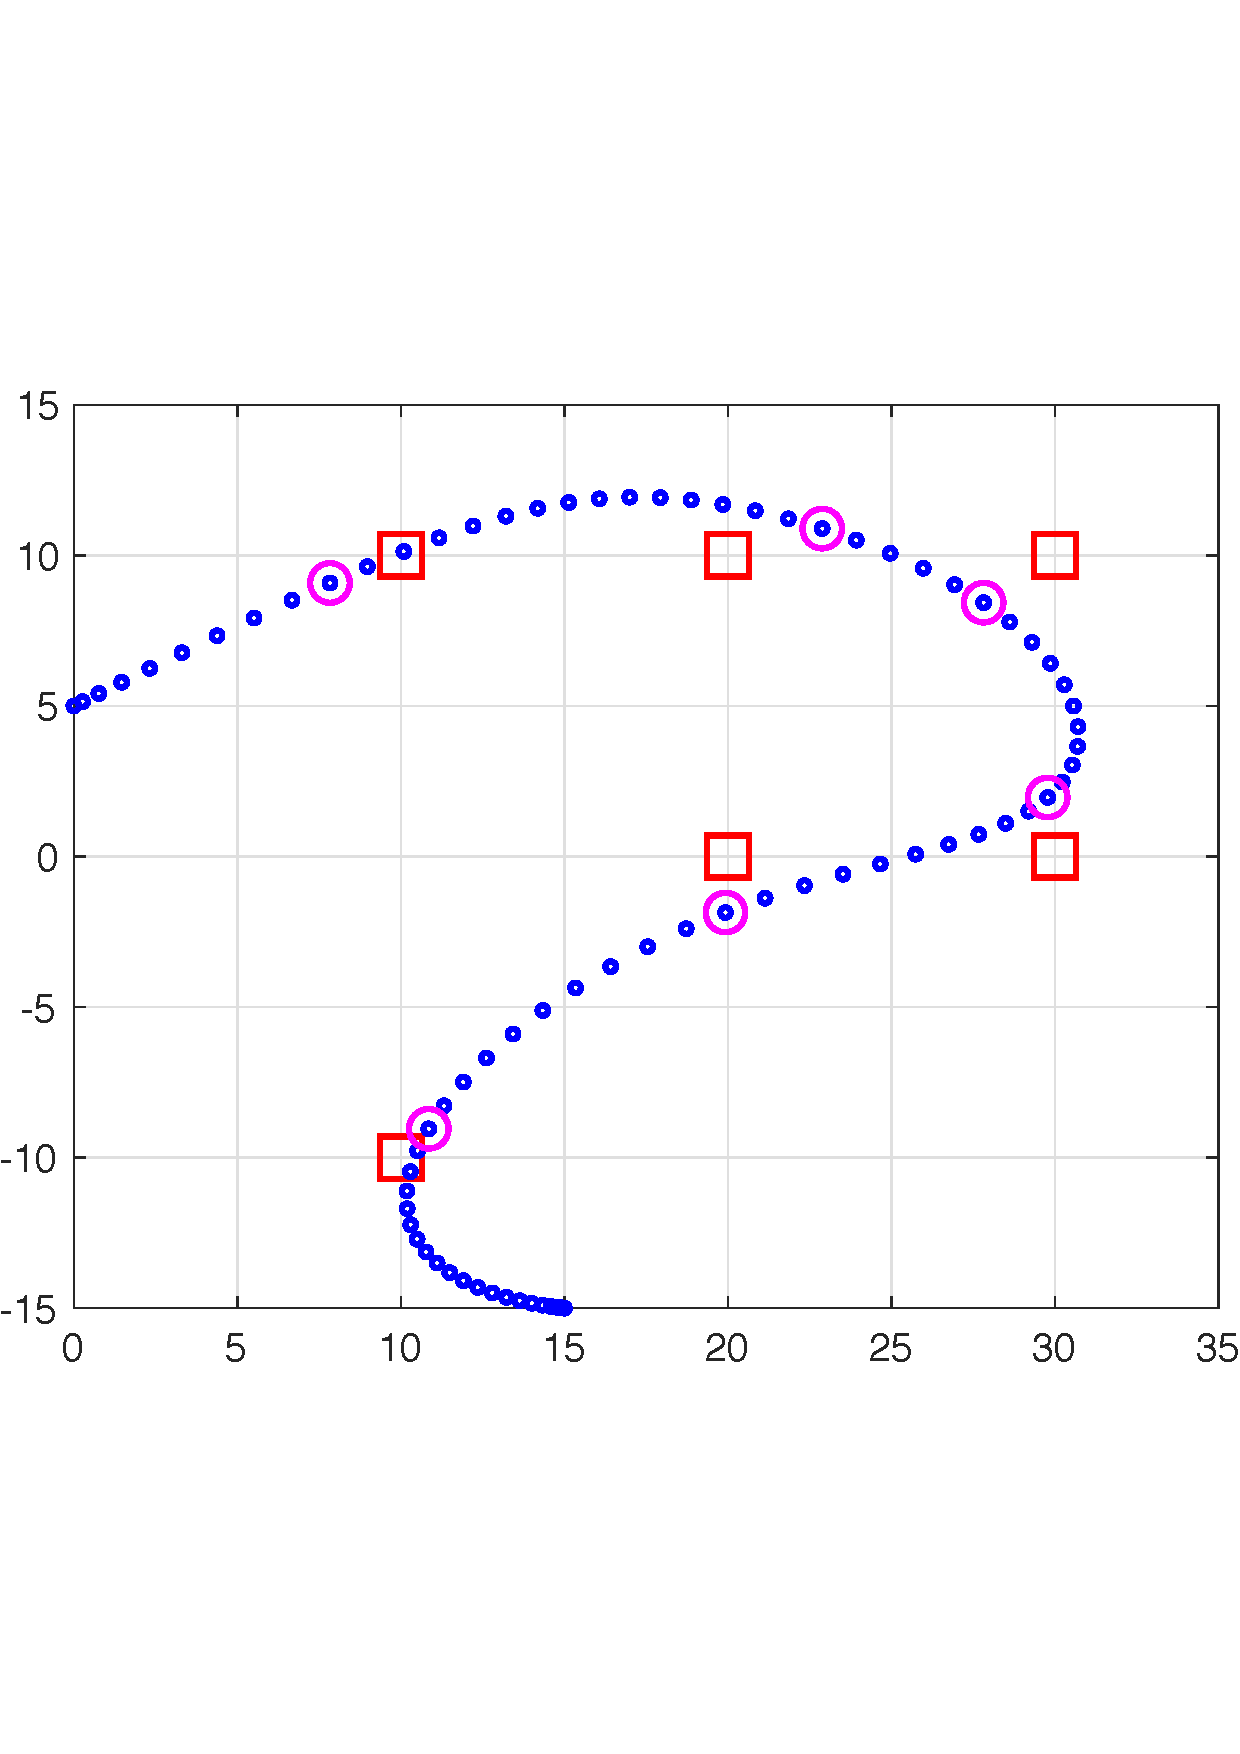
\includegraphics[width=10cm]{examplefig1.pdf}} \caption{Positions of the robot from $t = 0$ to $t = T$ are the small blue circles; the positions at appointed times $\tau_k$, for $1 \leq k \leq K$, are the large magenta circles. The waypoints are the red squares. Case $\lambda = 10^{-1}$ with $\ell_2^2$ regularizer. } \label{fig1}
\end{figure}

Figure~\ref{fig2} show two pictures, side by side.
\begin{figure}
\hfill
\subfigure[Caption A]{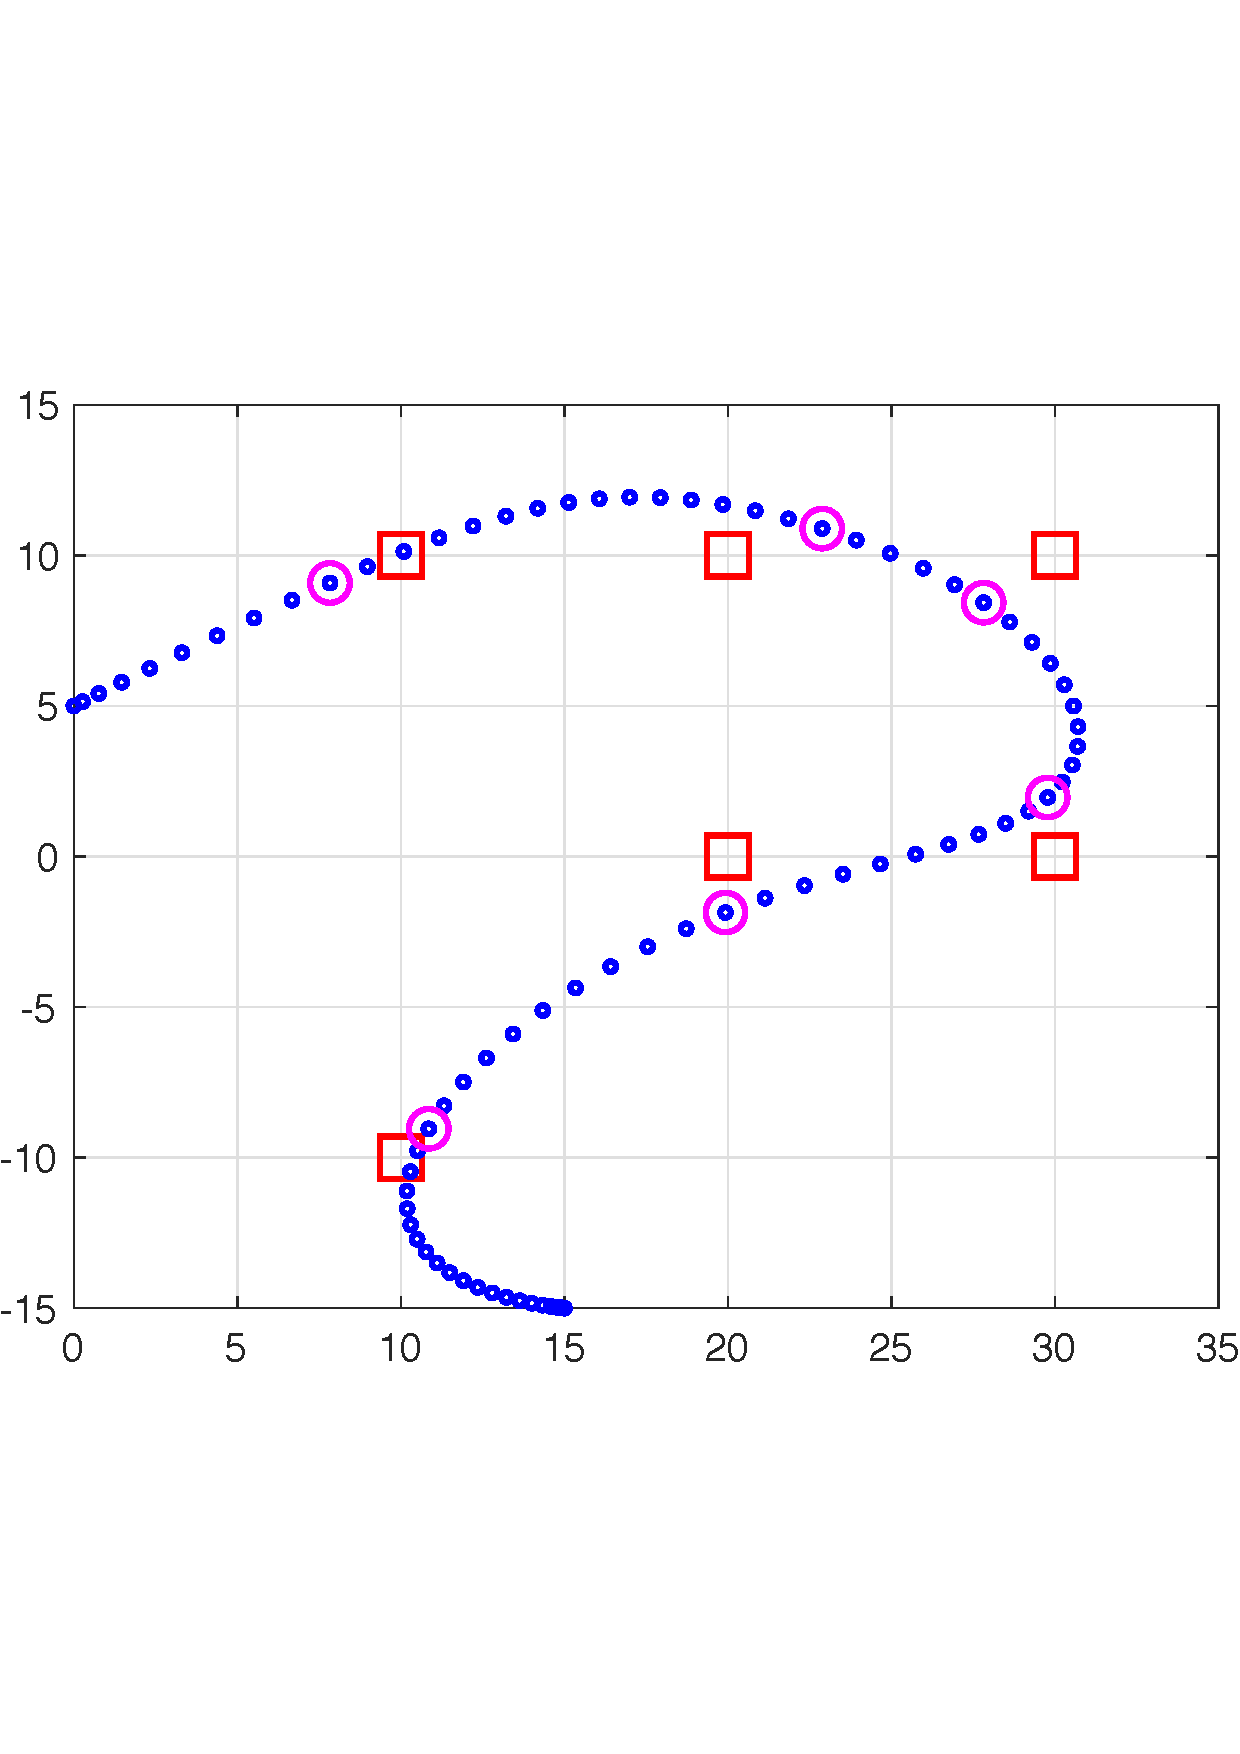
\includegraphics[width=7cm]{examplefig1.pdf}}
\hfill
\subfigure[Caption B]{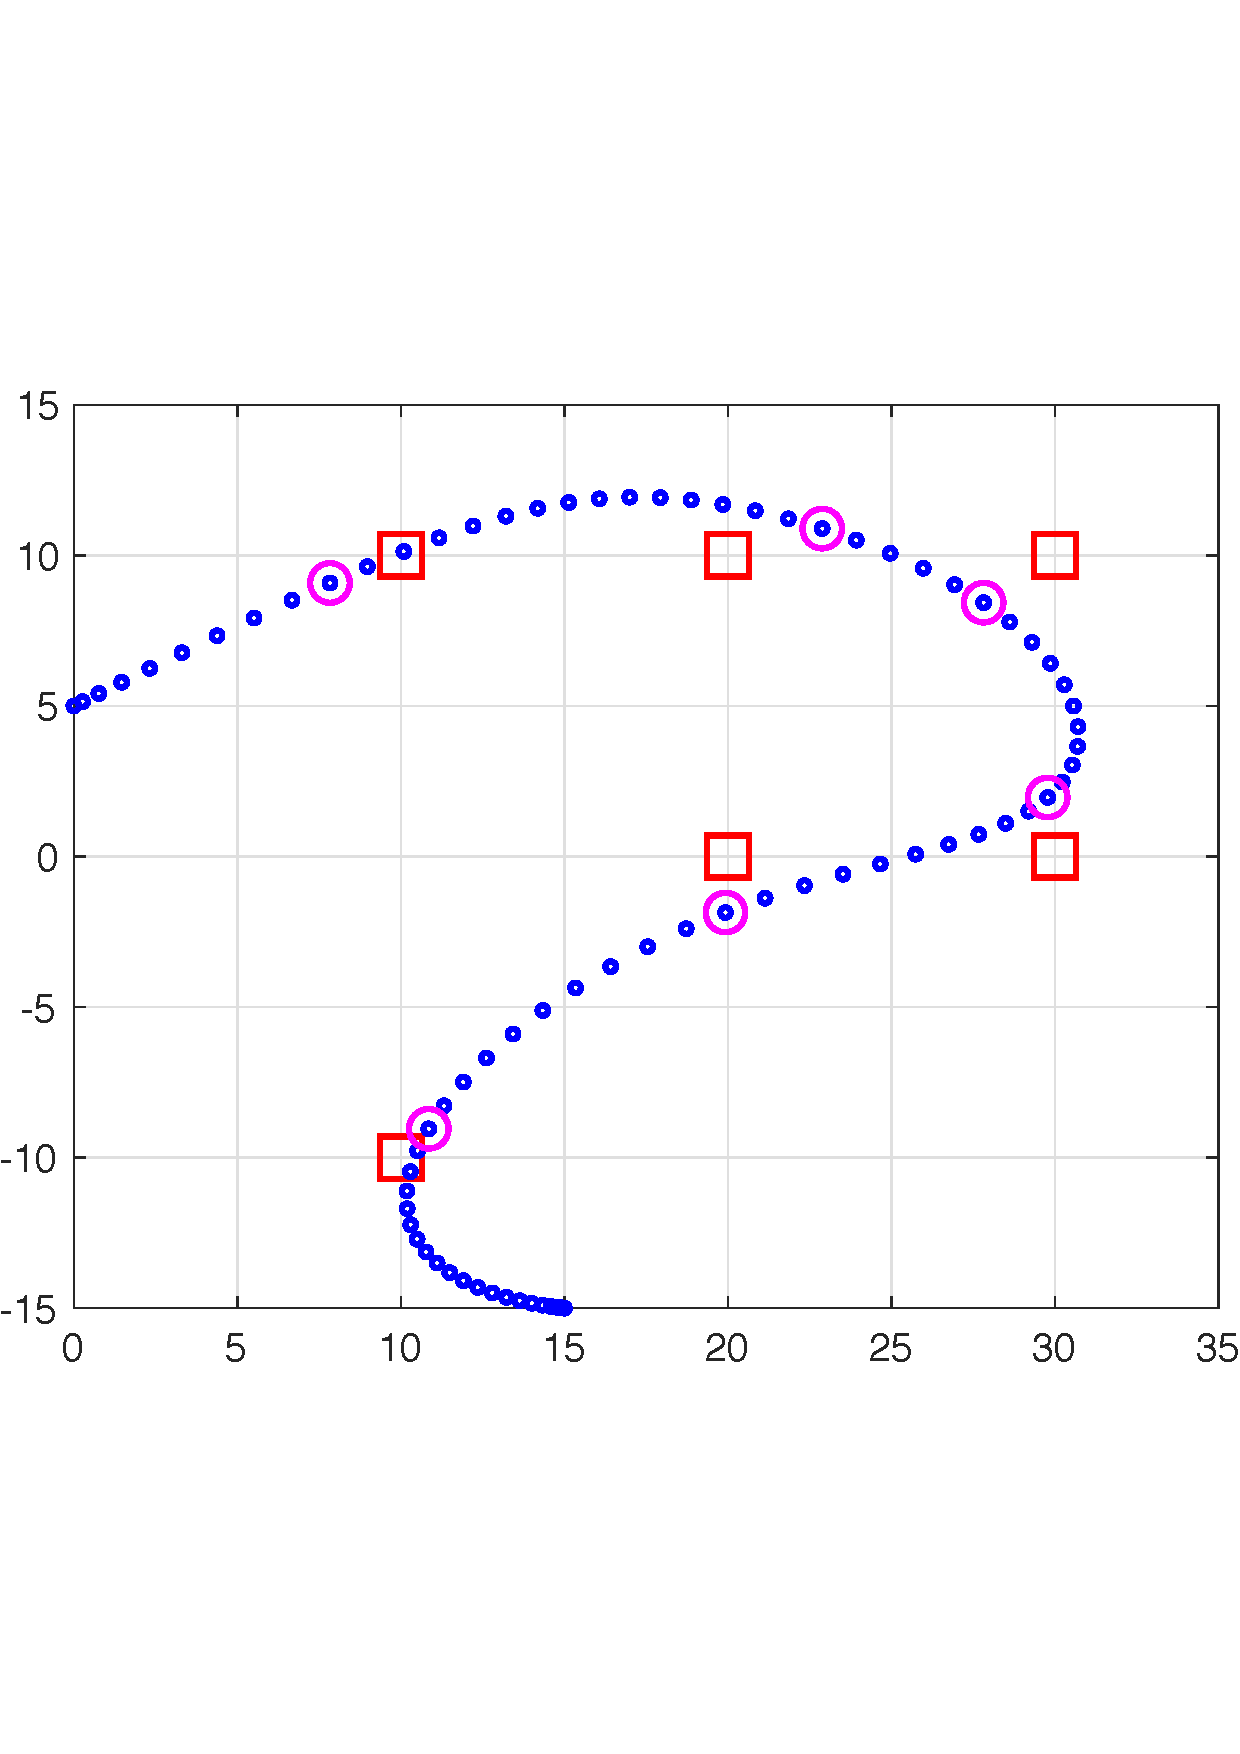
\includegraphics[width=7cm]{examplefig1.pdf}}
\hfill
\caption{A figure with two pictures.}
\label{fig2}
\end{figure}

Sometimes, a table is the most useful way to give information. See table~\ref{tab1} for an example.

\begin{table}[h!]
  \begin{center}
    \label{tab:table1}
    \begin{tabular}{l|c|r} 
      $\lambda$ & $d_1$ & $d_2$ \\
      \hline
      $10^{-3}$ & $25.98$ & $0.03$ \\
      $10^{-2}$ & $18.97$ & $1.05$ \\
      $10^{-1}$ & $16.65$ & $2.79$ \\
    \end{tabular}
  \end{center}
      \caption{An example of a table.} \label{tab1}
\end{table}


In the first part of the project,  we play with the following basic question: How should we act on a robot so that it transfers from a given position to another desired position? 

We solve three separate variations of this basic question:
\begin{itemize}
\item (section~\ref{S:variationA}) how should we act on the robot---using simple control signals---so that the robot also passes, as close as possible, to certain intermediate \textit{points} along its journey?
\item (section~\ref{S:variationB}) how should we act on the robot---using simple control signals---so that the robot also passes, as close as possible, to certain intermediate \textit{regions} along its journey? 
\item (section~\ref{S:variationC}) how should we act on  the robot so that it also passes \textit{exactly} on as many intermediate points as possible?
%\item (section~\ref{S:variationD}) how should we act on the robot---using simple control signals---so that the robot also passes, as close as possible, to certain intermediate points and \textit{avoids} a forbidden region?
\end{itemize}


\section{Variation A: approximate intermediate points and simple control signals} \label{S:variationA}

Section~\ref{sec:setup} states the problem in words, and each section~\ref{regA}, ~\ref{regB}, and ~\ref{regC} explores a different way to formulate it as an optimization problem.

\subsection{Problem statement} \label{sec:setup}

We are interested in the behaviour of the robot over the finite time horizon~$\{ 0, 1, 2, \ldots, T \}$. 

\paragraph{Where is our robot? The state of the robot.}
The position of the robot at time~$t$ in $\{ 0, 1, \ldots, T \}$ is denoted by $p(t)$; its velocity, by $v(t)$. Because we consider a robot moving in a plane, the position and velocity vectors are two-dimensional, that is, $p(t) \in {\mathbf R}^2$ and $v(t) \in {\mathbf R}^2$ for $0 \leq t \leq T$. The \textit{state} $x(t)$ of the robot at time $t$ is  $$x(t) = \begin{bmatrix} p(t) \\ v(t) \end{bmatrix}.$$
Note that $x(t)$ is a four-dimensional vector: $x(t) \in {\mathbf R}^4$, for $0 \leq t \leq T$.

\paragraph{How do we act on the robot? The control signal.}
We act on the robot by applying a force at each time $t$ in $\{ 0, 1, \ldots, T-1 \}$. (In practice, these forces are applied by the motor in the robot.) The force that we apply at time~$t$,  denoted by $u(t)$, is two-dimensional, that is, $u(t) \in {\mathbf R}^2$ for $0 \leq t \leq T-1$. The sequence of forces applied throughout time, $\{ u(t) \colon t = 0, \ldots, T-1 \}$, is  the \textit{control signal}. 

\paragraph{How does the robot move? The dynamics of the robot.}
Each time we apply a force to the robot, thereby pushing it, we change its state (position and velocity). More precisely, if $x(t)$ is the state of the robot at time~$t$ and we apply the force $u(t)$ at time~$t$, then the state of the robot changes to \begin{equation} x(t+1) = A x(t) + B u(t), \label{dynamics} \end{equation}
where $A \in {\mathbf R}^{4\times 4}$ and $B \in {\mathbf R}^{4\times 2}$ are known matrices. These matrices depend on physical constants such as the mass of the robot and the drag coefficient of the environment (to know more details on how to obtain $A$ and $B$, see slides 17---24 in Part 1, ``The art of formulating optimization problems''). 
For this project, consider $$A = \begin{bmatrix*}[r] 1 & 0 & 0.1 & 0 \\ 0 & 1 & 0 & 0.1 \\ 0 & 0 & 0.9 & 0 \\ 0 & 0 & 0 & 0.9 \end{bmatrix*} \quad \text{and} \quad B = \begin{bmatrix*}[r] 0 & 0 \\ 0 & 0 \\ 0.1 & 0 \\ 0 & 0.1 \end{bmatrix*}.$$


\paragraph{What do we want the robot to do?} We have several wishes:

\begin{itemize}

\item \textbf{Wish 1: transfer.} We wish the robot, which is resting at $t = 0$ in a given initial position $p_\text{initial} \in {\mathbf R}^2$, to transfer to a desired position  at time $t = T$, denoted $p_\text{final} \in {\mathbf R}^2$, and to rest there. That is, the initial state $x(0)$ of the robot is given by $x( 0 ) = x_\text{initial}$, where $x_\text{initial} = ( p_\text{initial} , 0 ) \in {\mathbf R}^4$, and we wish the final state $x(T)$ to be $x(T) = x_\text{final}$, where $x_\text{final} = ( p_\text{final}, 0 ) \in {\mathbf R}^4$;

\item \textbf{Wish 2: bounded control.} Because the motor of the robot is limited, we can apply forces only up to a certain magnitude, say $U_\text{max}$. That is, we wish  the control signal to satisfy $\left\| u(t) \right\|_2 \leq U_\text{max}$ for $0 \leq t \leq T-1$, where $$\left\| x \right\|_2 = \left( x_1^2  + \cdots + x_n^2 \right)^{1/2}$$ is the usual Euclidean norm of a vector $x$ in ${\mathbf R}^n$ with $x = ( x_1, \ldots, x_n )$. This norm is also commonly called the $\ell_2$ norm;

\item \textbf{Wish 3: waypoints.} As the robot transfers from its initial position to its final position, we also would like it to  pass as close as possible to certain intermediate locations---called \textit{waypoints}---at given appointed times. For example, we could wish the robot to get data from information sources at those locations, via wireless; because wireless signals  weaken with distance, the closer the robot is to each of the locations at the appointed times, the better.

The set of waypoints is $\{ w_1, \ldots, w_K \}$, and the associated set of appointed times is $\{ \tau_1, \ldots, \tau_K \}$. Hence our wish is to have the position of the robot at each time $\tau_k$ to be close to $w_k$, that is, $p( \tau_k ) \simeq w_k$ for $1 \leq k \leq K$; 

\item \textbf{Wish 4: simple control.} Finally, we wish to have a ``simple'' control signal, that is, a control signal that is constant, or, at least, a control signal that changes just a few times during the time horizon $\{0, 1, \ldots, T-1 \}$. This means that we wish to have $u(t) = u(t-1)$ for most values of $t$ in $\{ 1, \ldots, T- 1\}$.

\end{itemize}

\subsection{The $\ell_2^2$ regularizer} \label{regA}

We now convert the wish list at the end of section~\ref{sec:setup} into an optimization problem. We encode the first two wishes (transfer and bounded control) as constraints of the optimization problem; to deal with the last two wishes (waypoints and simple control), we create a cost function that penalizes deviations from those wishes. 

\paragraph{Optimization problem.} We formulate the problem as follows:
\begin{equation} \begin{array}[t]{ll} \underset{x, u}{\text{minimize}} & \sum_{k = 1}^K \left\| E x( \tau_k ) - w_k \right\|_2^2 + \lambda \sum_{t = 1}^{T-1} \left\| u(t) - u(t-1) \right\|_2^2 \\
\text{subject to} & x(0) = x_\text{initial} \\ & x(T) = x_\text{final}  \\ & \left\| u(t) \right\|_2 \leq U_\text{max}, \quad \text{ for } 0 \leq t \leq T-1 \\ & x(t+1) = A x(t) + B u(t), \quad \text{ for } 0 \leq t \leq T-1.\end{array} \label{prob1} \end{equation}

The variables to optimize are $x$ and $u$, where $x$ stands for the sequence of states of the robot, $\left( x(0), x(1), \ldots, x(T) \right)$, and $u$ stands for the sequence of control signals we apply, $\left( u(0), u(1), \ldots, u(T-1) \right)$. 

Thus, in the optimization problem~\eqref{prob1}, we are composing the state trajectory and the control signal, jointly.
Of course, these variables are linked by the physics of the problem, that is, the robot dynamics; this link is expressed by the last constraint in~\eqref{prob1}.

\paragraph{The first two wishes (transfer and bounded control).} The first two wishes are enforced by the first three constraints, which force the initial and final state to be the given ones and the magnitude of the control signal to be upper bounded by the given maximum admissible value.

\paragraph{The last two wishes (waypoints and simple control).}


The matrix~$E$ in the cost function of~\eqref{prob1} is $$E = \begin{bmatrix} 1 & 0 & 0 & 0 \\ 0 & 1 & 0 & 0 \end{bmatrix},$$
that is, $E x(\tau_k)$ gives the position of the robot at time~$\tau_k$: $E x(\tau_k) = p( \tau_k )$. Hence the first sum in the cost function, \begin{equation} \sum_{k = 1}^K \left\| E x(\tau_k) - w_k \right\|_2^2, \label{E:1} \end{equation} penalizes deviations of the position of the robot from the waypoints, at the given appointed times. This sum takes care of the third wish (waypoints). 

The fourth wish (simple control) is dealt with  by the last sum in the cost function,
\begin{equation}
\sum_{t = 1}^{T-1} \left\| u(t) - u(t-1) \right\|_2^2,
\label{regu}
\end{equation}
which penalizes deviations of the control signal at time~$t$ from its previous value at time~$t-1$, across the time horizon.
The sum in~\eqref{regu} is the \textit{regularizer}. We call it a $\ell_2^2$ regularizer because it uses the \textit{square} of the $\ell_2$ norm of the control increments.

The two sums~\eqref{E:1} and~\eqref{regu} are blended additively in the cost function of~\eqref{prob1} by a weight $\lambda > 0$, the \textit{regularization parameter}. Increasing $\lambda$ gives more importance to the fourth wish, therefore playing down the third wish; decreasing $\lambda$ does the opposite.

\paragraph{Constants.} For problem~\eqref{prob1}, consider $T = 80$, $p_\text{initial} = ( 0, 5 )$, and $p_\text{final} = ( 15, -15 )$. Also, consider the $K = 6$ waypoints $$w_1 = \begin{bmatrix*}[r] 10 \\ 10 \end{bmatrix*}, w_2 = \begin{bmatrix*}[r] 20 \\ 10 \end{bmatrix*}, w_3  = \begin{bmatrix*}[r] 30 \\ 10 \end{bmatrix*}, w_4 = \begin{bmatrix*}[r] 30 \\ 0 \end{bmatrix*}, w_5 = \begin{bmatrix*}[r] 20 \\ 0 \end{bmatrix*}\text{ and }w_6 = \begin{bmatrix*}[r] 10 \\ -10 \end{bmatrix*},$$
with appointed times $$\tau_1 = 10, \tau_2 = 25, \tau_3 = 30, \tau_4 = 40, \tau_5 = 50, \text{ and }\tau_6 = 60.$$

The maximum control magnitude  is $U_{\max} = 100$.

\vspace*{4ex}

\noindent\fcolorbox{black}{lightgray}{
    \parbox{\textwidth}{ \textbf{Task 1.} Use  the software {\tt CVX} from {\tt http://cvxr.com/cvx} to solve problem~\eqref{prob1} for $\lambda \in \{ 10^{-3}, 10^{-2}, 10^{-1}, 10^0, 10^1, 10^2, 10^3 \}$. So, you solve $7$ problems (one per value of $\lambda$ in the list). After each problem is solved, do the following: \begin{enumerate}[(a)]
    \item plot the optimal positions of the robot from $t = 0$ to $t = T$, marking its positions at the appointed times $\tau_k$, for $1 \leq k \leq K$;
    \item plot the optimal control signal $u(t)$, where $u(t) = ( u_1(t), u_2(t) )$, from $t = 0$ to $t = T-1$;
    \item report how many times the optimal control signal changes from $t = 1$ to $t = T-1$: we say that the control signal changes at time $t$ if $\left\| u(t) - u(t-1) \right\|_2 > 10^{-6}$; this tells us how much the fourth wish of a simple control is ignored;
    \item report the mean deviation from the waypoints, defined as \begin{equation} \frac{1}{K} \sum_{k = 1}^K \left\| E x(\tau_k) - w_k \right\|_2, \label{meanwaydev} \end{equation} which tells us how much the third wish (waypoints) is ignored.
    \end{enumerate}
    
    }
}

\vspace*{2ex}

\paragraph{Example.}
So that you can have an example to check your code, we give the answer for the case $\lambda = 10^{-1}$: Figure~\ref{fig1} answers part (a), and figure~\ref{fig2} answers part (b). The answer to part (c) is $79$, that is, the optimal control signal changes at each time instant $t \in \{ 0, 1, \ldots, T- 1 \}$ (recall that $T = 80$); you can also confirm this from figure~\ref{fig2}. Finally, the answer to part (d), the mean waypoint deviation~\eqref{meanwaydev}, is $2.1958$.

\begin{figure}[!htbp]
\centerline{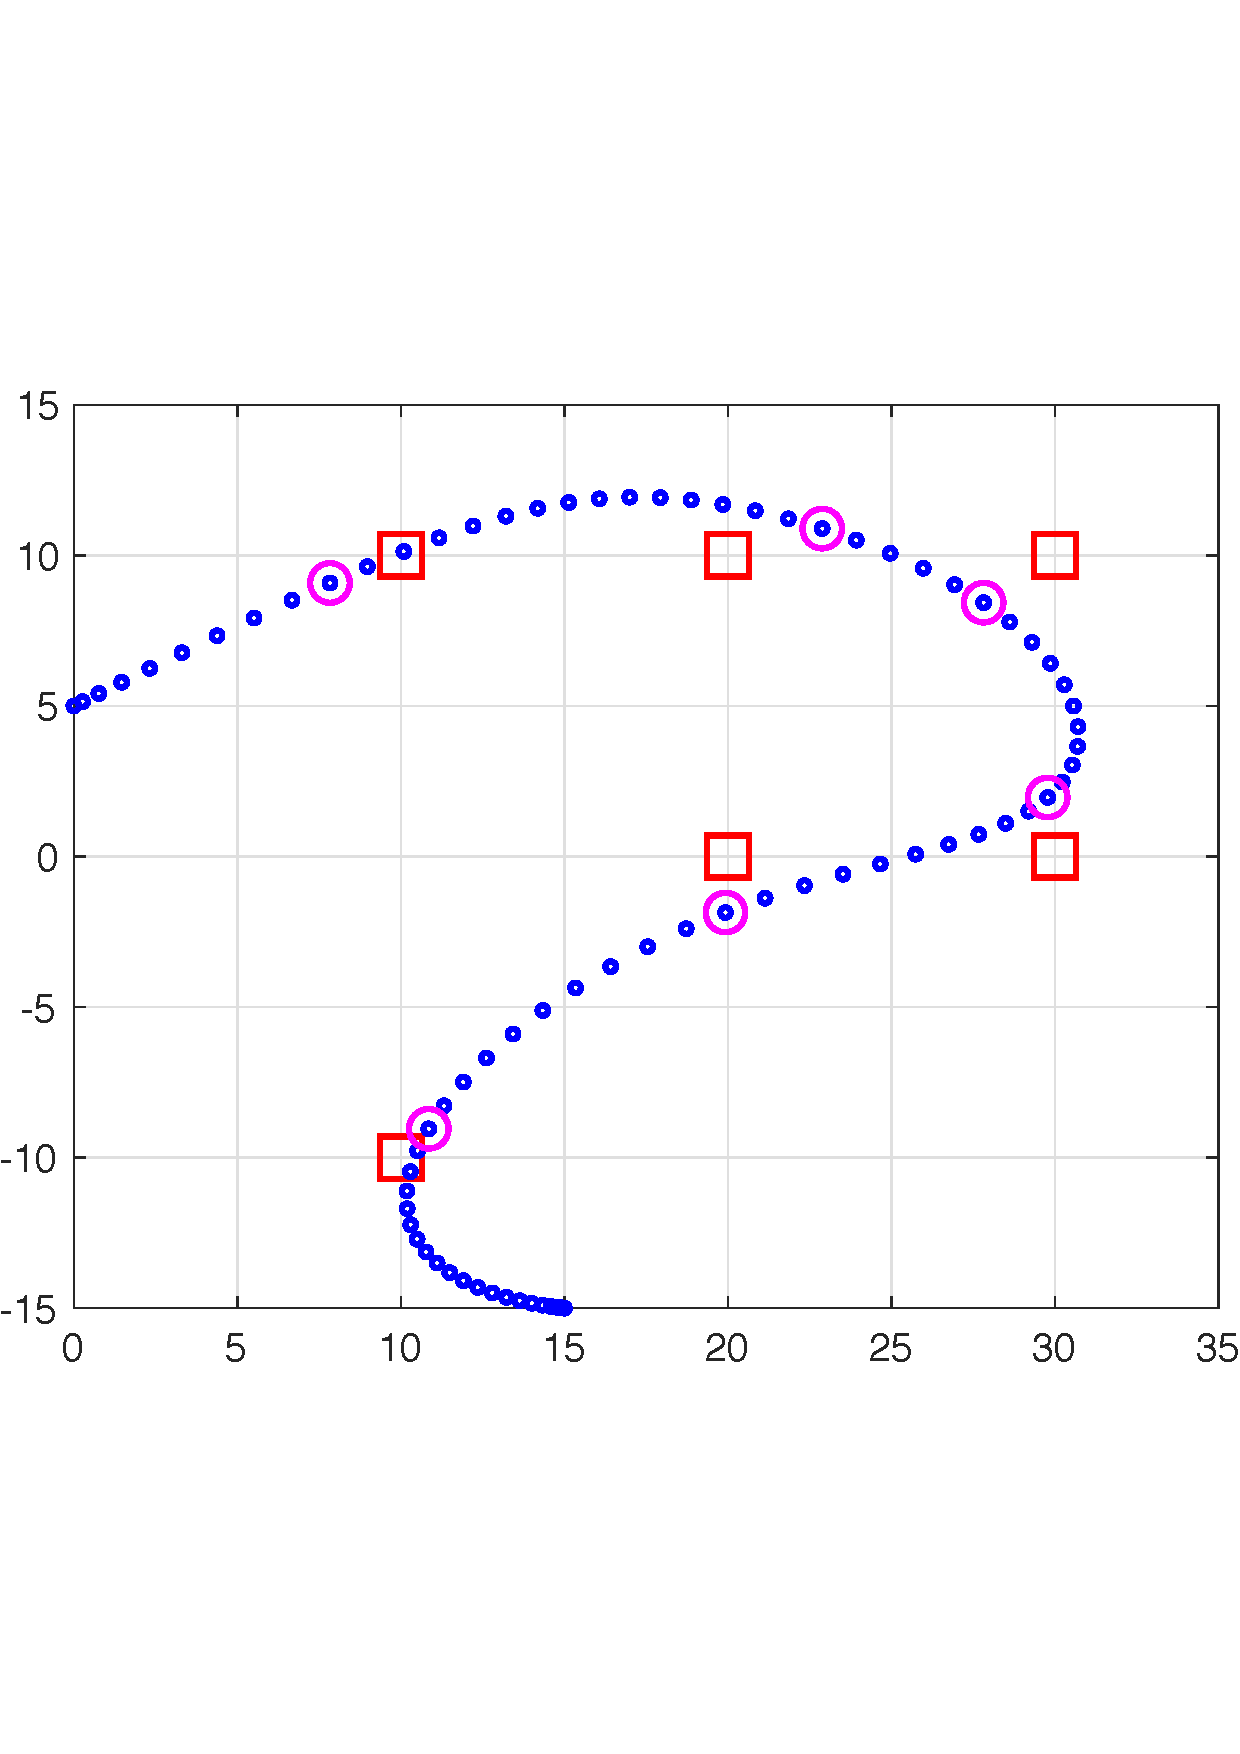
\includegraphics[width=10cm]{examplefig1.pdf}} \caption{Positions of the robot from $t = 0$ to $t = T$ are the small blue circles; the positions at appointed times $\tau_k$, for $1 \leq k \leq K$, are the large magenta circles. The waypoints are the red squares. Case $\lambda = 10^{-1}$ with $\ell_2^2$ regularizer---see problem~\eqref{prob1}. } \label{fig1}
\end{figure}

\begin{figure}[!htbp]
\centerline{\includegraphics[width=10cm]{examplefig2.pdf}} \caption{The two components, $u_1(t)$ and $u_2(t)$, of the control signal $u(t)$ from $t = 0$ to $t = T-1$. Case $\lambda = 10^{-1}$ with $\ell_2^2$ regularizer---see problem~\eqref{prob1}.} \label{fig2}
\end{figure}

\subsection{The $\ell_2$ regularizer} \label{regB}

We now remove the square of the $\ell_2$ regularizer in~\eqref{prob1} and formulate the problem as follows:
\begin{equation} \begin{array}[t]{ll} \underset{x, u}{\text{minimize}} & \sum_{k = 1}^K \left\| E x( \tau_k ) - w_k \right\|_2^2 + \lambda \sum_{t = 1}^{T-1} \left\| u(t) - u(t-1) \right\|_2 \\
\text{subject to} & x(0) = x_\text{initial} \\ & x(T) = x_\text{final}  \\ & \left\| u(t) \right\|_2 \leq U_\text{max}, \quad \text{ for } 0 \leq t \leq T-1 \\ & x(t+1) = A x(t) + B u(t), \quad \text{ for } 0 \leq t \leq T-1.\end{array} \label{prob2} \end{equation}

\vspace*{2ex}

\noindent\fcolorbox{black}{lightgray}{
    \parbox{\textwidth}{ \textbf{Task 2.} Redo task 1 for the optimization problem~\eqref{prob2}. 
    }
}

\paragraph{Example.} We give the answer for $\lambda = 10^{-1}$, which you should reproduce. The answers to parts (a) and (b) are in figures~\ref{fig3} and~\ref{fig4}, respectively. The answer to part (c) is $11$, and the answer to part (d) is $0.7021$.

\begin{figure}[!htbp]
\centerline{\includegraphics[width=10cm]{examplefig1b.pdf}} \caption{Positions of the robot from $t = 0$ to $t = T$ are the small blue circles; the positions at appointed times $\tau_k$, for $1 \leq k \leq K$, are the large magenta circles. The waypoints are the red squares. Case $\lambda = 10^{-1}$ with $\ell_2$ regularizer---see problem~\eqref{prob2}. } \label{fig3}
\end{figure}

\begin{figure}[!htbp]
\centerline{\includegraphics[width=10cm]{examplefig2b.pdf}} \caption{The two components, $u_1(t)$ and $u_2(t)$, of the control signal $u(t)$ from $t = 0$ to $t = T-1$. Case $\lambda = 10^{-1}$ with $\ell_2$ regularizer---see problem~\eqref{prob2}.} \label{fig4}
\end{figure}


\subsection{The $\ell_1$ regularizer} \label{regC}

As a final way to tackle  the fourth wish (simple control), we use a regularizer based on the $\ell_1$ norm. For a vector $x \in {\mathbf R}^n$ with $x = ( x_1, \ldots, x_n )$, the $\ell_1$ norm is $$\left\| x \right\|_1 = | x_1 | + \cdots + | x_n |.$$


We formulate the problem as follows:
\begin{equation} \begin{array}[t]{ll} \underset{x, u}{\text{minimize}} & \sum_{k = 1}^K \left\| E x( \tau_k ) - w_k \right\|_2^2 + \lambda \sum_{t = 1}^{T-1} \left\| u(t) - u(t-1) \right\|_1 \\
\text{subject to} & x(0) = x_\text{initial} \\ & x(T) = x_\text{final}  \\ & \left\| u(t) \right\|_2 \leq U_\text{max}, \quad \text{ for } 0 \leq t \leq T-1 \\ & x(t+1) = A x(t) + B u(t), \quad \text{ for } 0 \leq t \leq T-1.\end{array} \label{prob3} \end{equation}

\vspace*{2ex}

\noindent\fcolorbox{black}{lightgray}{
    \parbox{\textwidth}{ \textbf{Task 3.} Redo task 1 for the optimization problem~\eqref{prob3}. 
    }
}

\paragraph{Example.} We give the answer for $\lambda = 10^{-1}$. Parts (a) and (b) are in answered in figures~\ref{fig5} and~\ref{fig6}, respectively. The answer to part (c) is $14$, and the answer to part (d) is $0.8863$.

\begin{figure}[!htbp]
\centerline{\includegraphics[width=10cm]{examplefig1c.pdf}} \caption{Positions of the robot from $t = 0$ to $t = T$ are the small blue circles; the positions at appointed times $\tau_k$, for $1 \leq k \leq K$, are the large magenta circles. The waypoints are the red squares. Case $\lambda = 10^{-1}$ with $\ell_1$ regularizer---see problem~\eqref{prob3}. } \label{fig5}
\end{figure}

\begin{figure}[!htbp]
\centerline{\includegraphics[width=10cm]{examplefig2c.pdf}} \caption{The two components, $u_1(t)$ and $u_2(t)$, of the control signal $u(t)$ from $t = 0$ to $t = T-1$. Case $\lambda = 10^{-1}$ with $\ell_1$ regularizer---see problem~\eqref{prob3}.} \label{fig6}
\end{figure}

\vspace*{4ex}

\noindent\fcolorbox{black}{lightgray}{
    \parbox{\textwidth}{ \textbf{Task 4.} Comment on what you have observed from Tasks 1 to 3 (for example, compare the impact of the three regularizers on the optimal control signal that they each induce).
    }
}

\section{Variation B: approximate intermediate regions and simple control signals} \label{S:variationB}

In section~\ref{S:variationA}, we want the robot to pass near certain intermediate points, at appointed times. 

\paragraph{Disks.} Suppose now that we want the robot to pass near certain intermediate regions, namely,  disks. A disk, denoted $D(c, r)$, is a set of the form $\{ x \in {\mathbf R}^2\, :\, \left\| x - c \right\|_2 \leq r \}$,  where $c \in {\mathbf R}^2$ is the center of the disk and $r$ its radius.

We consider $K$ intermediate disks $\{ D(c_k, r_k) \, :\, 1 \leq k \leq K \}$ along with appointed times $\{ \tau_k \,:\, 1 \leq k \leq K \}$. In this variation, we want the robot to be as close as possible to disk $D(c_k, r_k)$ at time $\tau_k$.  We don't care whether the robot is close to the \textit{center} of the disk; only whether it is close to the \textit{whole} disk (for example, if the robot is inside the disk at time $\tau_k$, we don't care whether the robot is near the center or near the boundary). 
Thus, we care only about $d\left( p(\tau_k), D(c_k, r_k) \right)$, where $d\left(p, D(c,r) \right)$ is the distance of the point $p \in {\mathbf R}^2$ to the disk $D(c, r)$: $$d\left(p, D(c,r) \right) = \min\left\{ \left\| p - y \right\|_2\, : \, y \in D(c, r) \right\}.$$


\vspace*{2ex}


\noindent\fcolorbox{black}{lightgray}{
    \parbox{\textwidth}{ \textbf{Task 5.} Using simple geometric arguments, give a  closed-form expression for $d\left( p,D(c,r) \right)$.
    }
}

\paragraph{Problem formulation.} For this variation, we formulate the following optimization problem:
\begin{equation} \begin{array}[t]{ll} \underset{x, u}{\text{minimize}} & \sum_{k = 1}^K d\left(  E x( \tau_k ), D(c_k, r_k) \right)^2  +  \lambda \sum_{t = 1}^{T-1} \left\| u(t) - u(t-1) \right\|_2\\
\text{subject to} & x(0) = x_\text{initial} \\ & x(T) = x_\text{final}  \\ & \left\| u(t) \right\|_2 \leq U_\text{max}, \quad \text{ for } 0 \leq t \leq T-1 \\ & x(t+1) = A x(t) + B u(t), \quad \text{ for } 0 \leq t \leq T-1.\end{array} \label{P:prob4} \end{equation}



\paragraph{Constants.} For problem~\eqref{P:prob4}, consider $\lambda = 10^{-1}$. The set of intermediate $K = 6$ disks is $\{ D(c_k, r_k) \, :\, \text{ for } 1 \leq k \leq K \}$, where 
$$c_1 = \begin{bmatrix*}[r] 10 \\ 10 \end{bmatrix*}, c_2 = \begin{bmatrix*}[r] 20 \\ 10 \end{bmatrix*}, c_3  = \begin{bmatrix*}[r] 30 \\ 10 \end{bmatrix*}, c_4 = \begin{bmatrix*}[r] 30 \\ 0 \end{bmatrix*}, c_5 = \begin{bmatrix*}[r] 20 \\ 0 \end{bmatrix*}\text{ and }c_6 = \begin{bmatrix*}[r] 10 \\ -10 \end{bmatrix*},$$
with appointed times $$\tau_1 = 10, \tau_2 = 25, \tau_3 = 30, \tau_4 = 40, \tau_5 = 50, \text{ and }\tau_6 = 60.$$ Note that the centers of the disks are the previous waypoints. Take all the radiuses of the disks to be $2$. All other constants are as in section~\ref{S:variationA}.

\vspace*{4ex}


\noindent\fcolorbox{black}{lightgray}{
    \parbox{\textwidth}{ \textbf{Task 6.} Use the software ${\tt CVX}$ to solve problem~\eqref{P:prob4}. After you solve the problem, do the following:
    \begin{enumerate}[(a)]
    \item plot the optimal positions of the robot from $t = 0$ to $t = T$, marking its positions at the appointed times $\tau_k$, for $1 \leq k \leq K$;
    \item plot the optimal control signal $u(t)$, where $u(t) = ( u_1(t), u_2(t) )$, from $t = 0$ to $t = T-1$;
    \item report how many times the optimal control signal changes from $t = 1$ to $t = T-1$; 
    \item report the mean deviation from the waypoints (defined in~\eqref{meanwaydev});     
    \item comment on the results from (a)-(d), as you compare them with those you obtained in Task 1. (Note that Task 1 considered waypoints, which can be seen as disks with radius zero.)
    \end{enumerate}


    
    }
}

\section{Variation C: exact intermediate points} \label{S:variationC}

For this  variation, we drop the wish for a simple control signal. But we become more serious about the waypoints. 

\paragraph{Exact waypoints.} In section~\ref{S:variationA} we wish the robot to pass \textit{approximately} on certain waypoints at appointed times, that is, we want the position $p( \tau_k )$ of the robot at an appointed time $\tau_k$ to be close to its associated waypoint $w_k$: $p( \tau_k ) \simeq w_k$. 

In this section, however, we want the robot to pass on waypoints \textit{exactly}: We want to have \begin{equation} p( \tau_k ) = w_k, \label{E:wish} \end{equation} for as many waypoints $k \in \{ 1, \ldots, K \}$ as possible. When the robot passes exactly on a given waypoint, we say that the robot \textit{captures} that waypoint. Hence we wish the robot to capture as many waypoints as possible along its transfer.


\subsection{Two uninteresting formulations}

\paragraph{A feasibility formulation.} Why simply not enforce the equalities~\eqref{E:wish} for $1 \leq k \leq K$? That is, why not try to capture all the waypoints? This leads to the following formulation:
\begin{equation} \begin{array}[t]{ll} \underset{x, u}{\text{minimize}} & 0 \\
\text{subject to} & x(0) = x_\text{initial} \\ & x(T) = x_\text{final}  \\ & \left\| u(t) \right\|_2 \leq U_\text{max}, \quad \text{ for } 0 \leq t \leq T-1 \\ & x(t+1) = A x(t) + B u(t), \quad \text{ for } 0 \leq t \leq T-1, \\ & E x(\tau_k) = w_k, \quad \text{ for }1 \leq k \leq K. \end{array} \label{P:prob5a} \end{equation}
In~\eqref{P:prob5a} the cost function is identically zero. That's because there is nothing to optimize. We just want a control signal that makes the robot pass exactly on all the waypoints. A problem in which the cost function is identically zero is called a \textit{feasibility problem}: in such problems, we just want to find a point that is \textit{feasible}---a point that satisfies all the constraints.

\paragraph{Constants.} For problem~\eqref{P:prob5a} take $U_{\max} = 15$. Note that this constant has changed; previously, it was $100$, which means that we are dealing now with a robot with a weaker motor. All other constants are as in section~\ref{S:variationA}.

\vspace*{4ex}

\noindent\fcolorbox{black}{lightgray}{
    \parbox{\textwidth}{ \textbf{Task 7.} Use the software ${\tt CVX}$ to solve problem~\eqref{P:prob5a}. Explain what happens.
    }
}

\paragraph{A formulation too hard to solve.} Another possible formulation for this problem is as follows:
\begin{equation} \begin{array}[t]{ll} \underset{x, u}{\text{minimize}} & \sum_{k = 1}^K \phi\left( E x(\tau_k) - w_k \right)\\
\text{subject to} & x(0) = x_\text{initial} \\ & x(T) = x_\text{final}  \\ & \left\| u(t) \right\|_2 \leq U_\text{max}, \quad \text{ for } 0 \leq t \leq T-1 \\ & x(t+1) = A x(t) + B u(t), \quad \text{ for } 0 \leq t \leq T-1.\end{array} \label{P:prob5} \end{equation}
The function $\phi$ in~\eqref{P:prob5} outputs a zero if its argument is zero and outputs a one, otherwise. That is, we have $\phi\,:\,{\mathbf R}^2 \rightarrow {\mathbf R}$, with $$\phi(x) = \left\{ \begin{array}{ll} 0,  & \text{ if } x = 0, \\ 1, & \text{ if }x \neq 0. \end{array} \right.$$
In words,  the objective function in~\eqref{P:prob5} counts the number of waypoints that the robot misses. So, in problem~\eqref{P:prob5}, we look for the control signal that makes the robot miss as few waypoints as possible.

It turns out that problem~\eqref{P:prob5} is nonconvex and too hard to solve numerically. 

\vspace*{4ex}


\noindent\fcolorbox{black}{lightgray}{
    \parbox{\textwidth}{ \textbf{Task 8.} Show that the function $\phi$ is nonconvex.
    
    }
}


\vspace*{4ex}

In sections~\ref{S:variationC1}, \ref{S:variationC2}, and \ref{S:variationC3}, we explore convex formulations that approximate  problem~\eqref{P:prob5} and are easy to solve numerically.

\subsection{A $\ell_2^2$ formulation} \label{S:variationC1}

We start by replacing the function $\phi$ by a squared $\ell_2$ norm:
\begin{equation} \begin{array}[t]{ll} \underset{x, u}{\text{minimize}} & \sum_{k = 1}^K \left\| E x(\tau_k) - w_k \right\|_2^2 \\
\text{subject to} & x(0) = x_\text{initial} \\ & x(T) = x_\text{final}  \\ & \left\| u(t) \right\|_2 \leq U_\text{max}, \quad \text{ for } 0 \leq t \leq T-1 \\ & x(t+1) = A x(t) + B u(t), \quad \text{ for } 0 \leq t \leq T-1.\end{array} \label{P:prob6} \end{equation}

\paragraph{Constants.} For problem~\eqref{P:prob6} consider $U_{\max} = 15$.  All other constants are as in section~\ref{S:variationA}.

\vspace*{4ex}


\noindent\fcolorbox{black}{lightgray}{
    \parbox{\textwidth}{ \textbf{Task 9.} Use the software ${\tt CVX}$ to solve problem~\eqref{P:prob6}. After you solve the problem, do the following:
    \begin{enumerate}[(a)]
    \item plot the optimal positions of the robot from $t = 0$ to $t = T$, marking its positions at the appointed times $\tau_k$, for $1 \leq k \leq K$;
    \item plot the optimal control signal $u(t)$, where $u(t) = ( u_1(t), u_2(t) )$, from $t = 0$ to $t = T-1$;
    \item report how many waypoints are captured by the robot; consider that a waypoint $w_k$ is captured if the robot is sufficiently close to it at the appointed time $\tau_k$, namely, if $\left\| p( \tau_k) - w_k \right\|_2 \leq 10^{-6}$.
    \end{enumerate}
    
    }
    }

\subsection{A $\ell_2$ formulation} \label{S:variationC2}

Consider now that the function $\phi$ is replaced by a $\ell_2$ norm:
\begin{equation} \begin{array}[t]{ll} \underset{x, u}{\text{minimize}} & \sum_{k = 1}^K \left\| E x(\tau_k) - w_k \right\|_2 \\
\text{subject to} & x(0) = x_\text{initial} \\ & x(T) = x_\text{final}  \\ & \left\| u(t) \right\|_2 \leq U_\text{max}, \quad \text{ for } 0 \leq t \leq T-1 \\ & x(t+1) = A x(t) + B u(t), \quad \text{ for } 0 \leq t \leq T-1.\end{array} \label{P:prob7} \end{equation}

\paragraph{Constants.} For problem~\eqref{P:prob7} consider $U_{\max} = 15$.  All other constants are as in section~\ref{S:variationA}.


\vspace*{4ex}

\noindent\fcolorbox{black}{lightgray}{
    \parbox{\textwidth}{ \textbf{Task 10.} Redo task 9 for problem~\eqref{P:prob7}.
    
    }
    }



\subsection{The iterative reweighting technique} \label{S:variationC3}

An iterative technique for improving on the results of problem~\eqref{P:prob7} consists in solving reweighted versions of it. 
Specifically, each iteration of the technique takes a current guess $x^{(m)}$ and $u^{(m)}$  and produces a new one $x^{(m+1)}$ and $u^{(m+1)}$ by solving the following problem:
\begin{equation} \begin{array}[t]{ll} \underset{x, u}{\text{minimize}} & \sum_{k = 1}^K \frac{1}{\left\| E x^{(m)}(\tau_k) - w_k \right\|_2 + \epsilon} \left\| E x(\tau_k) - w_k \right\|_2 \\
\text{subject to} & x(0) = x_\text{initial} \\ & x(T) = x_\text{final}  \\ & \left\| u(t) \right\|_2 \leq U_\text{max}, \quad \text{ for } 0 \leq t \leq T-1 \\ & x(t+1) = A x(t) + B u(t), \quad \text{ for } 0 \leq t \leq T-1.\end{array} \label{P:prob8} \end{equation}

Note the weight $1 / \left( \left\| E x^{(m)}(\tau_k) - w_k \right\|_2 + \epsilon \right)$ for each term $k$ in the sum of the objective function of~\eqref{P:prob8} (in~\eqref{P:prob7}, these weights are all $1$). The constant $\epsilon$ is a very small positive number that prevents the denominator to be zero.

Solving~\eqref{P:prob8} gives $x^{(m+1)}$ and $u^{(m+1)}$. The technique is initialized with $x^{(0)}$ and $u^{(0)}$, the solution of problem~\eqref{P:prob7}. 

\paragraph{Constants.} For problem~\eqref{P:prob8} consider $U_{\max} = 15$ and $\epsilon = 10^{-6}$.  All other constants are as in section~\ref{S:variationA}.


\vspace*{4ex}

\noindent\fcolorbox{black}{lightgray}{
    \parbox{\textwidth}{ \textbf{Task 11.} Apply the reweighting  technique $M$ times, with $M = 10$; that is, solve problem problem~\eqref{P:prob8} for $m = 0, 1, \ldots, M-1$. For each value of $m$, do the following:
     \begin{enumerate}[(a)]
    \item plot the positions of the robot in $x^{(m)}$ from $t = 0$ to $t = T$, marking its positions at the appointed times $\tau_k$, for $1 \leq k \leq K$;
    \item plot the control signal $u^{(m)}(t)$, where $u^{(m)}(t) = \left( u_1^{(m)}(t), u_2^{(m)}(t) \right)$, from $t = 0$ to $t = T-1$;
    \item report how many waypoints are captured by the robot.
    \end{enumerate}
    
    
    }
    }
    
    
    \vspace*{4ex}

\noindent\fcolorbox{black}{lightgray}{
    \parbox{\textwidth}{ \textbf{Task 12.} What's the role of the weights in~\eqref{P:prob8}?
    
    
    }
    }


%\section{Variation D: approximate intermediate points, simple control signals, and forbidden region} \label{S:variationD}
\end{document}
